\chapter{Внедрение БШС на нефтегазовых месторождениях}\label{ch:ch1}


Цифровая трансформация является первостепенной задачей для развития нефтегазового комплекса. Переход производства к новой модели управления <<Индустрия 4.0>> позволит бизнесу сохранить лидирующие позиции и не утратить производственного потенциала  \cite{Eremin2020, Dmitrievskiy2020}. Неотъемлемой частью такой трансфомарции является внедрение беспроводных технологий \cite{Eremin2020, Dmitrievskiy2020, Eremin2019, Hiriyannaiah2020, Munirathinam2020, CarmenLucas-Estan2018}. 


Современные беспроводные широкополосные сети связи (БШС), обладая рядом преимуществ, нашли свое широкое применение в задачах мониторинга и управления различных   производственных или гражданских объектов, технологических установок, движущихся транспортных средств и т.п. К ряду таких преимуществ можно отнести возможность получения информации с любой точки контролируемой территории, быстрый ввод в эксплуатацию, сокращение капитальных затрат на создание и эксплуатацию сети, высокая гибкость, мобильность и масштабируемость. 


Нефтегазовые объекты часто расположены в труднодоступной местности на обширной территории в несколько киллометров. Данный фактор является ключевым преимуществом беспроводных технологий для развертывания по сравнению с кабельными коммуникациями.

Беспроводная связь в автоматизации промышленного производства способствует осуществлению производственных процессов более экономически эффективно, гибко и надежно, а также позволяет реализовывать новые концепции автоматизации \cite{Gost62657}. Для управления большими объемами на месторождениях применение применение беспроводных каналов связи в режиме 60/24/7, позволяюшая операторам принимать обоснованные управленческие решения, своевременно диагностировать и устранять неисправности, а также оптимизировать работу АСУ ТП в целом \cite{Dmitrievsky2021}.

Не маловажную роль на месторождениях играет безопасность. Технологические объекты на нефтяных или газовых месторождениях, оснащенных широкополосным подключением, позволяют соответствовать современным концепциям и требованиям в сфере безопасности персонала и безопасности имущества, включая охрану с использованием беспроводных камер видеонаблюдения. Для предоставления доступа к объекту могут использоваться дополнительные возможности, такие как считывание номерных знаков и распознавание лиц. А благодаря использованию тепловых камер можно контролировать риски отключения и перегрузки даже с помощью периодических снимков оборудования на промысле. 

Внедрение БШС особенно хорошо подходят для систем видеонаблюдения, поскольку позволяют расположить камеры там, где они нужны, а не там, где удобно для подключения к проводной сети.

В данном исследовании в рамках цифровой трансформации <<Индустрия 4.0>> представлены модели и методы оптимизации при проектировании беспроводных сетей на месторождениях  (Рисунок \cref{fig:industry4}).

\begin{figure}[h!]
  \centering
   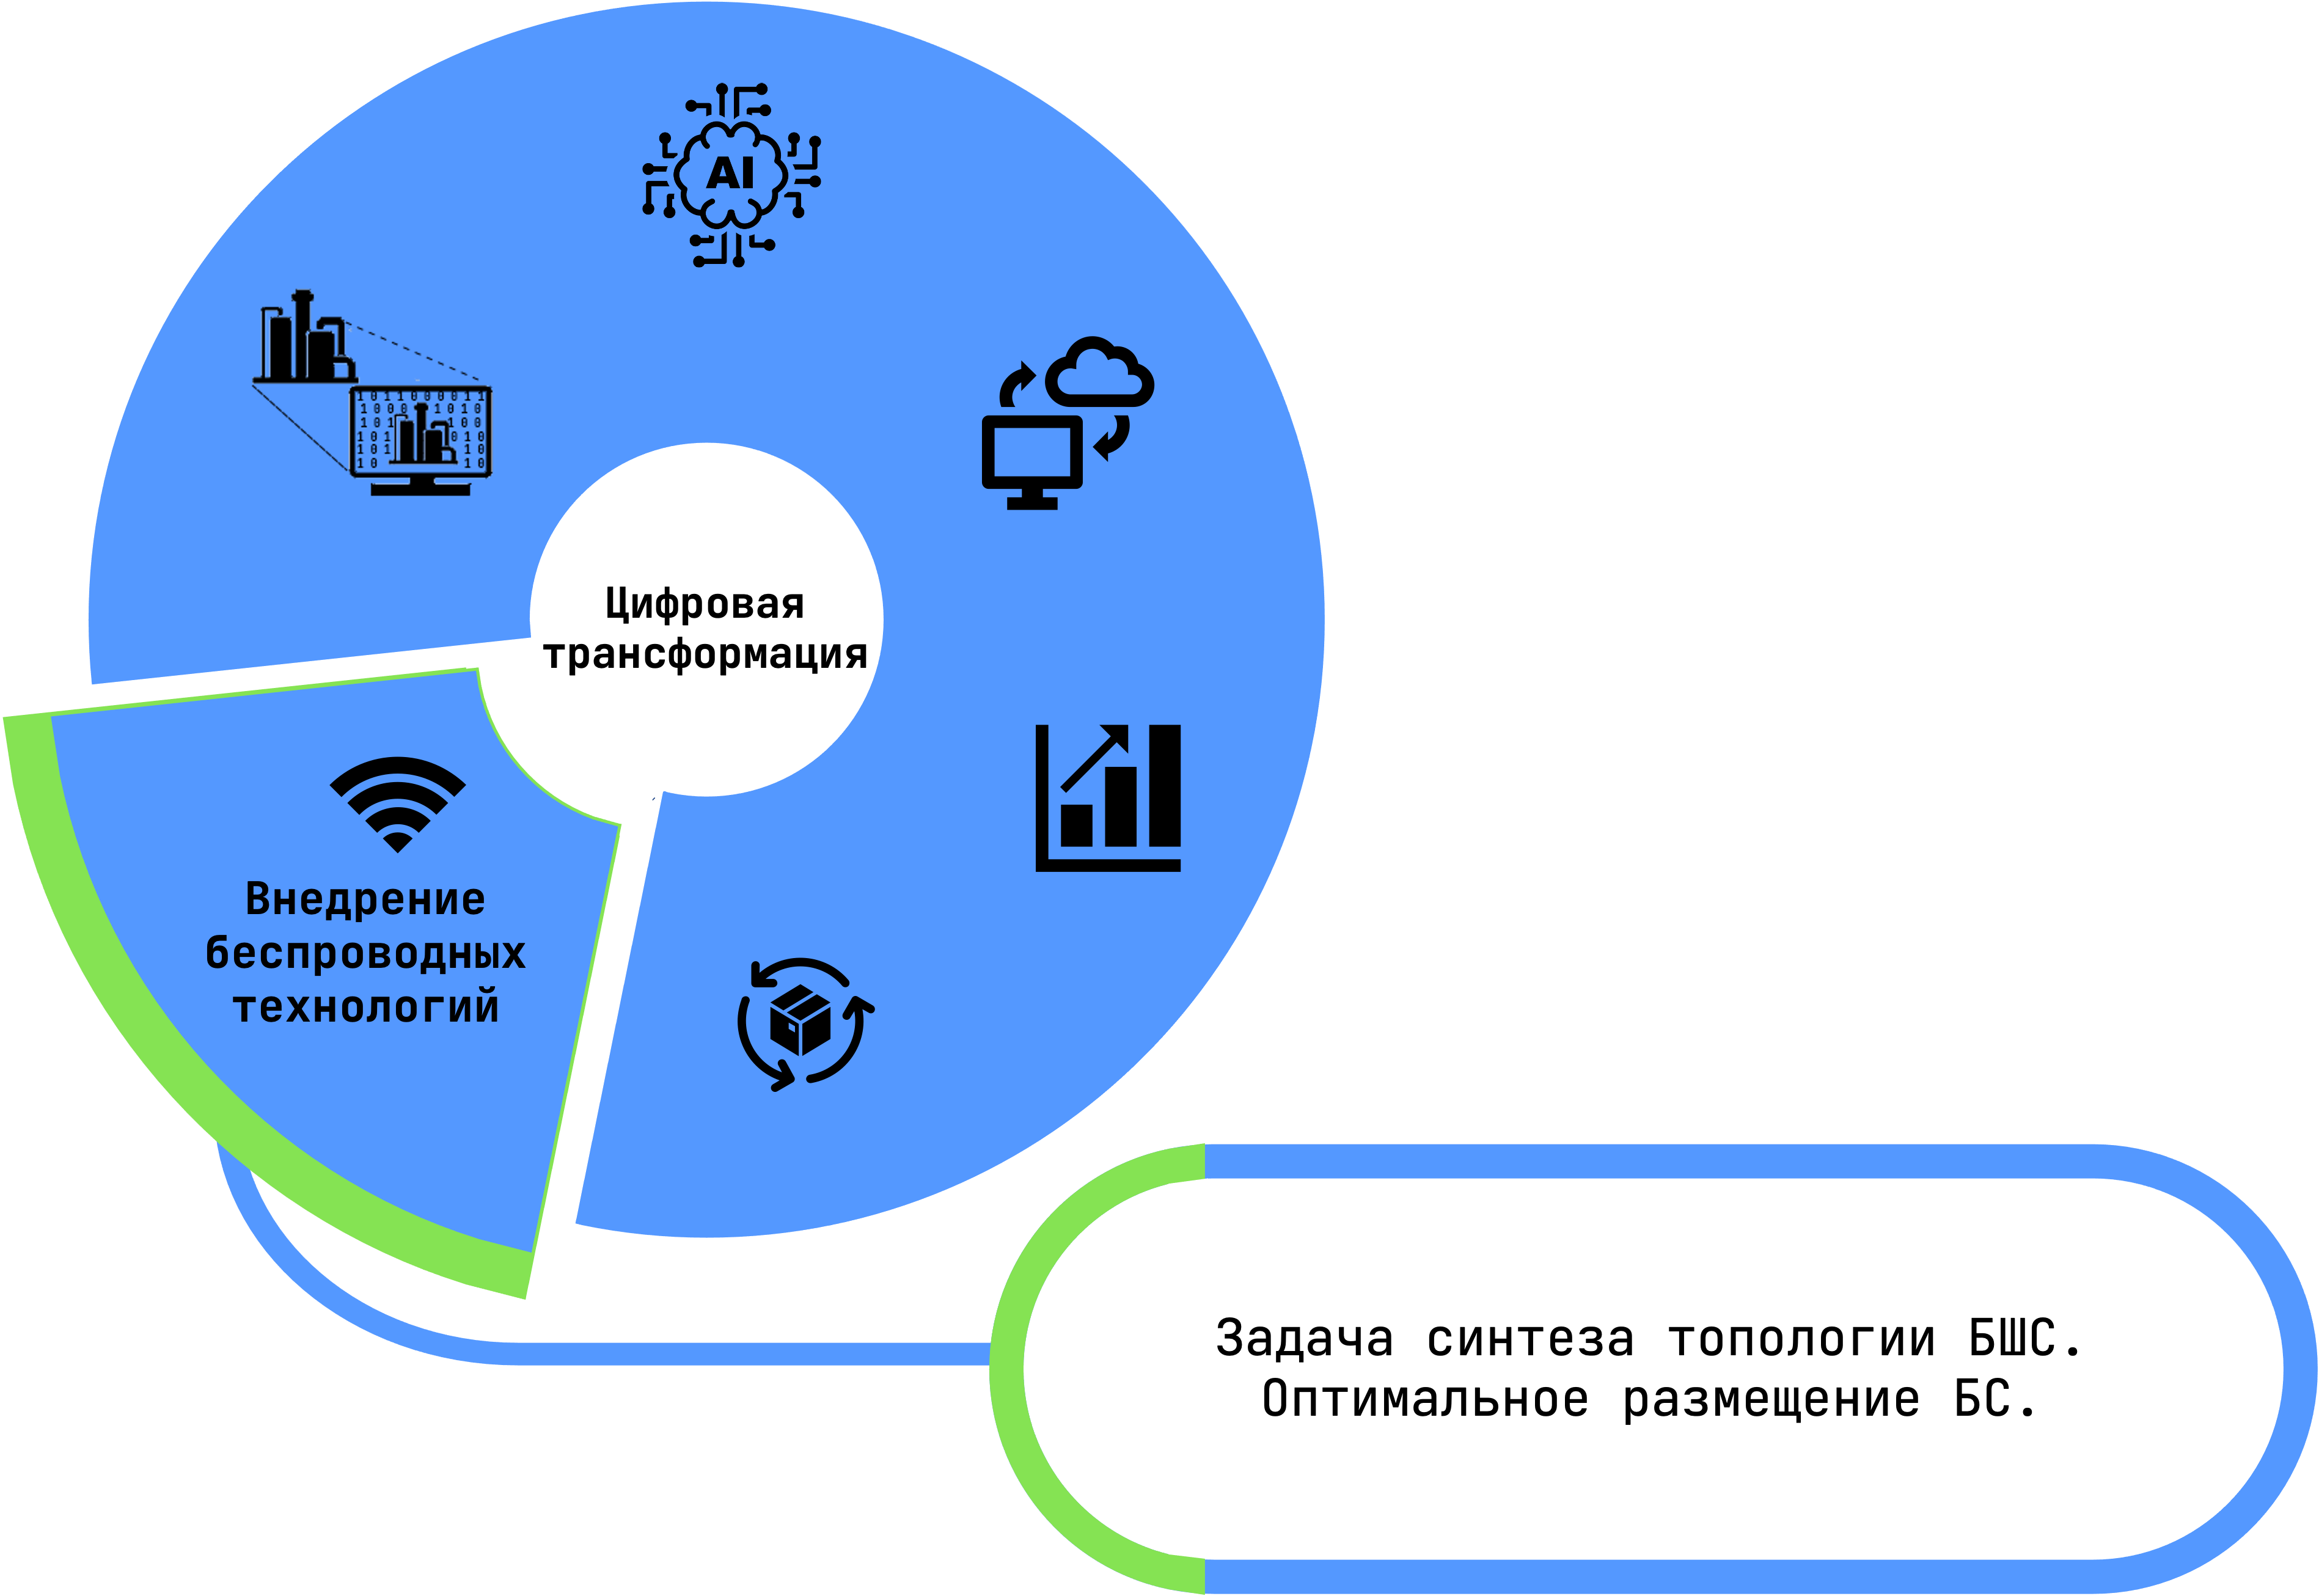
\includegraphics[width=1\textwidth]{industry4.png}
\caption{Задача синтеза топологии при проектировании БШС в рамках цифровой трансформации "Индустрия 4.0".}
\label{fig:industry4}
\end{figure}


\section{Этапы проектирования БШС}.


Для обеспечения высокого качества беспроводной связи необходимо проводить грамотное проектирование БШС. Существуют различные подходы к проектированию беспроводных сетей. Для одних задачей является максимальная зона покрытия, для других -- достижения максимальной производительности передачи данных, для третьих -- нахождения баланса между зоной охвата и производительностью \cite{Proletarsky}. В диссертации будут предложены модели и методы оптимального размещения базовых станций (БС) БШС, целью которых является максимальная зона охвата.  Процесс проектирования современной БШС, как правило, для такого подхода имеет следующие основные этапы (Рисунок \cref{fig:part1_design_stages}):

\begin{figure}[h!]
  \centering
   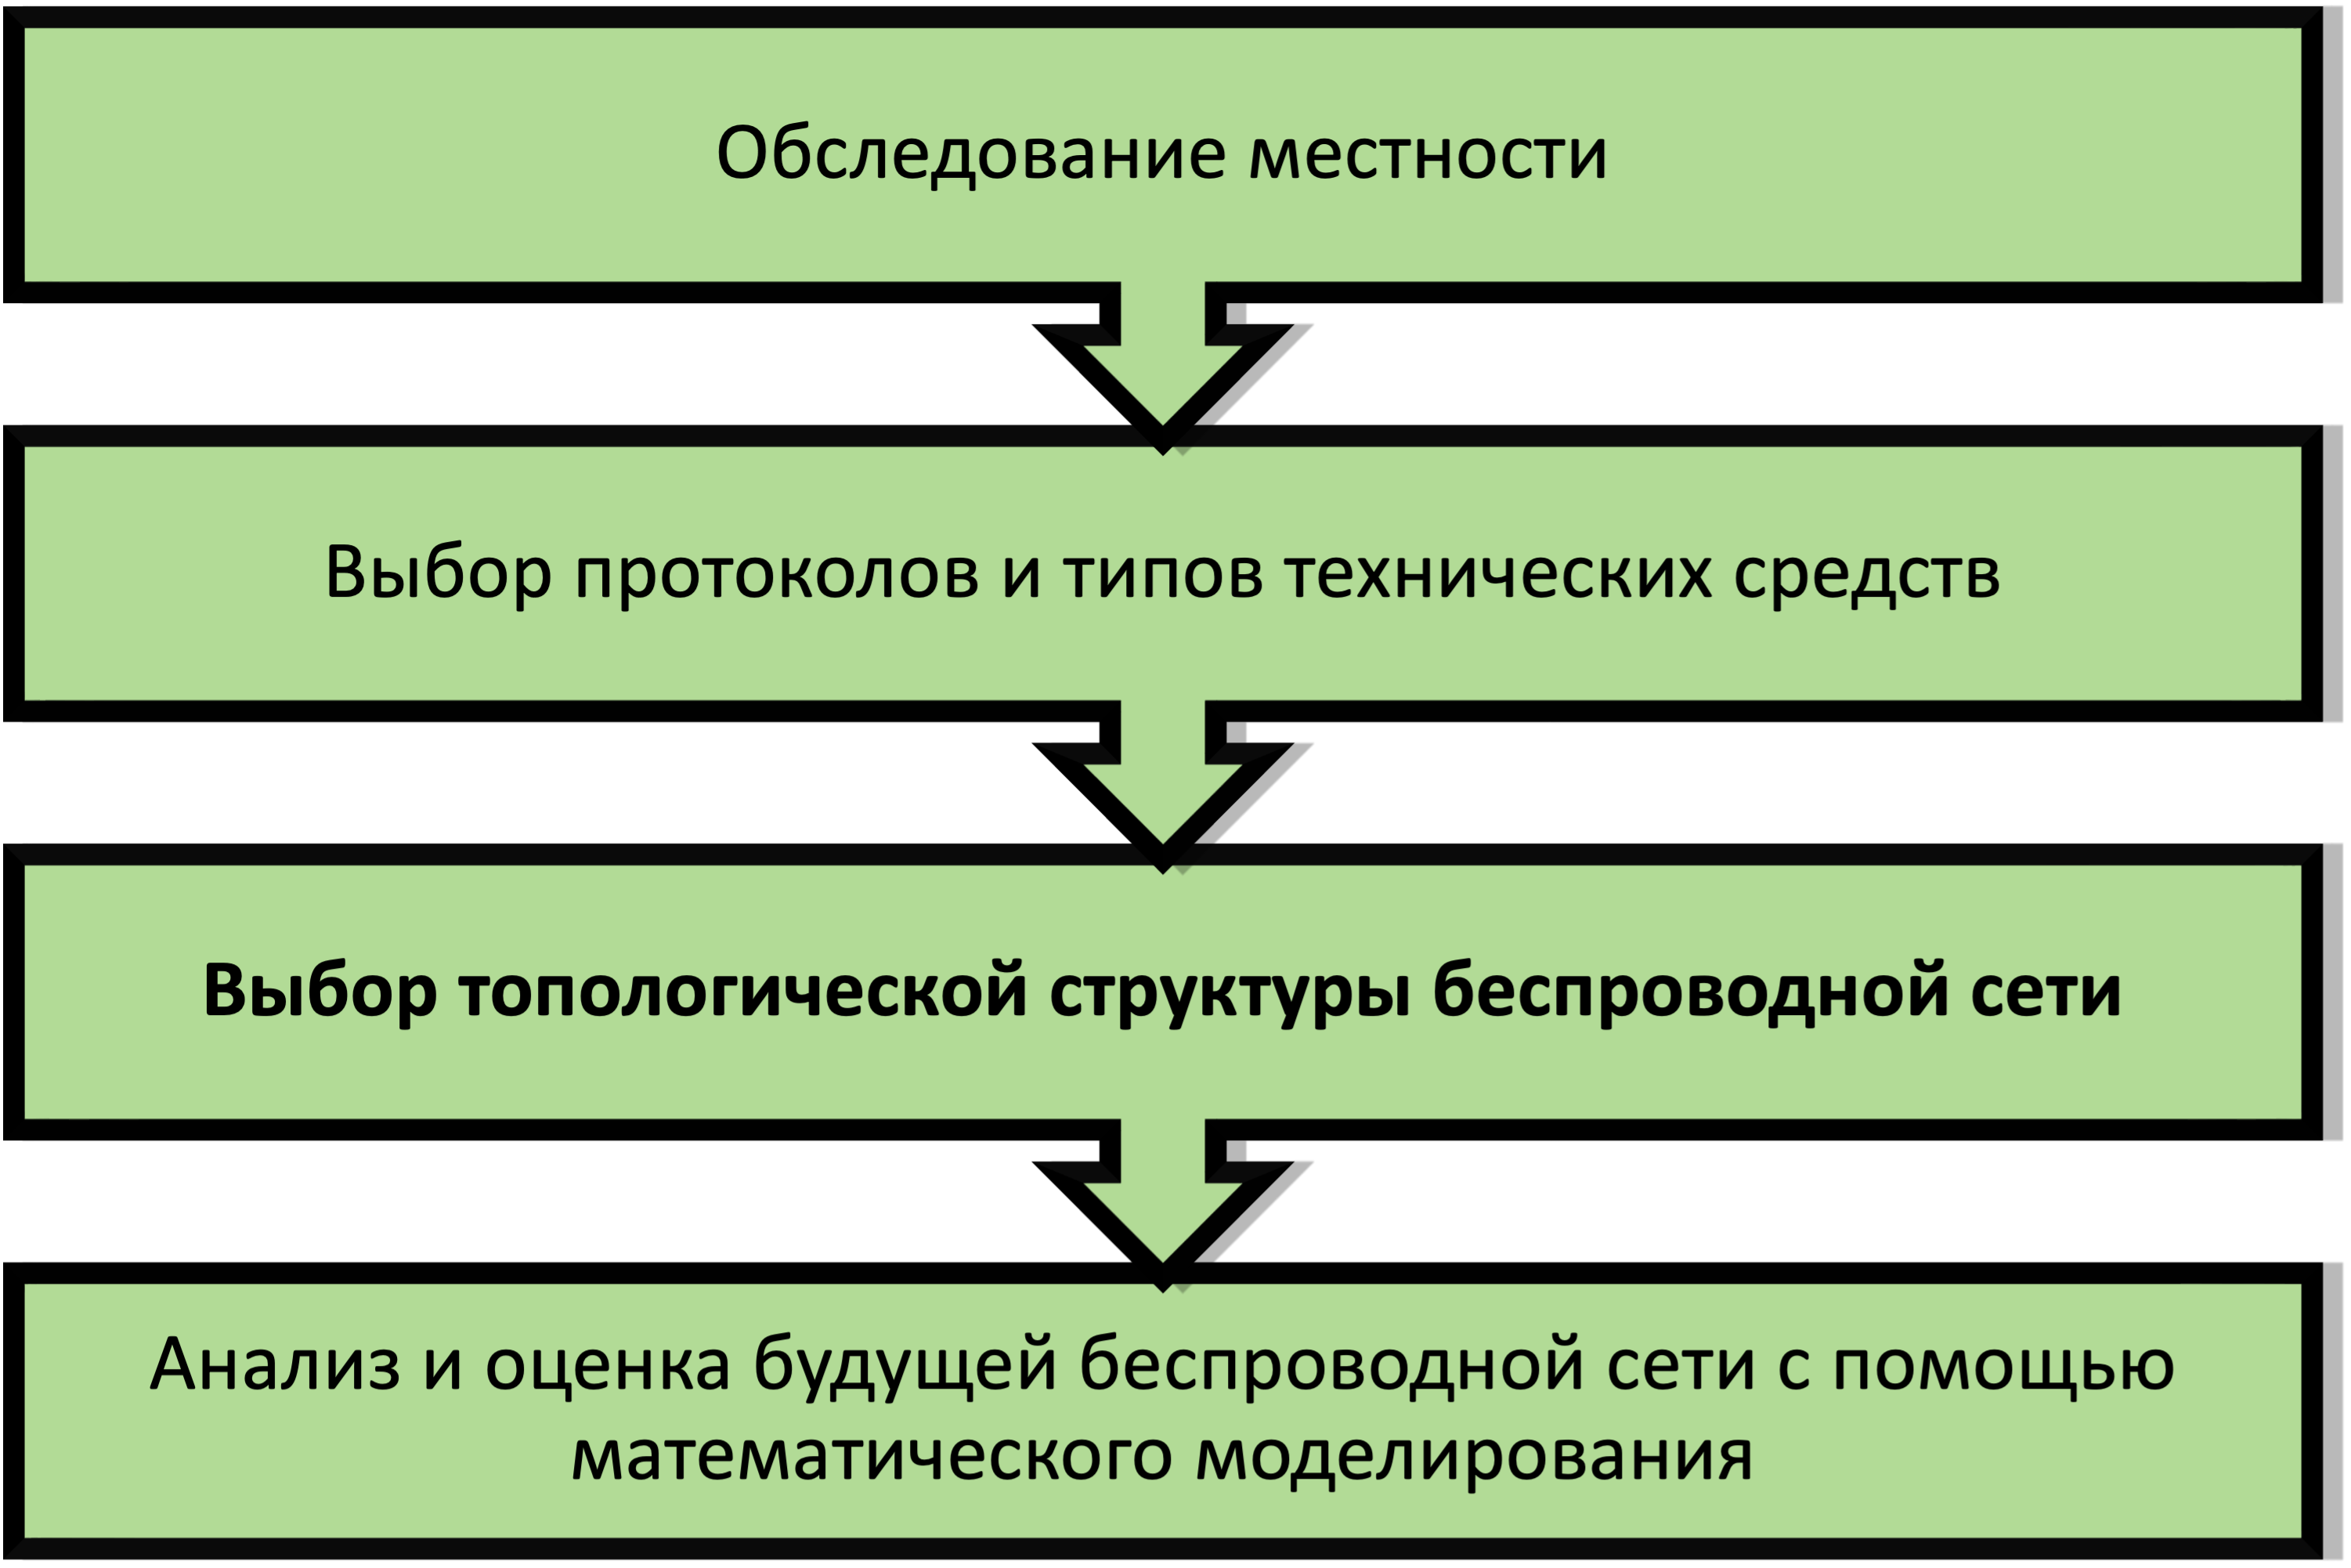
\includegraphics[width=0.8\textwidth]{design_stages.png}
\caption{Этапы проектирования БШС.}
\label{fig:part1_design_stages}
\end{figure}

Любое проектирование БШС всегда начинается с первоначального обследования местности. В данный этап входят задачи радиобследования и радиопланирования. оценки реальных размеров области контроля, наличие стационарных инженерно-технических соооружений, мешающих передачи сигнала, такими как металлические конструкции, перекрытия, стены и т.д. При развертывании БШС в открытой местности также немаловажную роль играет наличие перепада высот. В ходе выполнения комплекса работ на местности, определяются возможные точки размещения оборудования \cite{Dunaitsev2017}. На основе результатов данного этапа проводится выбор типо моделй оборудования для дальнейшего их размещения и организации сети.

Производительность и дальность действия беспроводных сетей не безграничны. При их проектировании стоит учитывать множество параметров: частота, скорость, мощность излучения \cite{Proletarsky}. На этапе выбора оборудования необходимо определиться с протоколом будущей БШС и  подготовить необходимый комплекс технических средств для развертывания будущей сети. БС является основопологающим устройством будущей сети, которая отвечает за покрытие задданной области. Покрытие в свою очередь зависит от мощности передатчика устройства, усиления антенн, чувствительности приемного устройства.


После определения множества возможных точек размещения БС на этапе обследования местности и выборе возможных типов и моделей оборудований можно переходить непосредственно к размещению БС и определению топологической структуры сети. Этап выбора топологической структуры будущей сети является ключевой проблемой данной диссертации. В рамках данной проблемы будут предложены модели и методы оптимального размещения БС для организации БШС.

После решения задачи синтеза топологии, для полученного размещения решаются задачи оценки характеристик производительности БШС. Для расчета оценок широко применяется аппарат теории массового осблуживания (ТМО). Примерами таких задач являются расчет надежности всех элементов сети \cite{Wankpo2020, Krishnamoorthy2021, Kozyrev2019}, оценка характеристик качества канала, вероятности потери пакетов, пропускной способности, времени доставки сообщений в сети \cite{Gorbunova2020, Larionov2019, Vishnevsky2016_Methods_of_performance, Vishnevsky2016_Review_of_methodology, Wang2017, Sandmann2012, Baumann2017}, оценка межкоцневой задержки сети \cite{Wang2017, Sandmann2012}. В работе \cite{Eremenko2013} рассматривают стохастическую модель марковской цепи для оценки качества предоставления информационных услуг передачи данных автоматизации систем управления технологическим процессов (АСУ ТП) в условиях помех и прерываний. Одним из современных направленией в исследовании характеристик производительности БШС является использование ТМО в совокупности с методами машинного обучения (МО) \cite{Lovas2021, SatyaHermanto2018}.

Описанная процедура проектиррования БШС является общей для большинства внедрения беспроводных коммуникационных сетей. В зависимости от конкретных целей, которые преследуют проектировщики, план работ может требовать содержание конкретных этапов и подзадач проектирования. В общем же случае проектирование БШС будет происходить согласно данной последовательности этапов. В изложенной концепции важным является представление места результатов исследования данной диссертации в глобальной задаче комплексного проектирования.

\section{Определение расчетных параметров БШС, необходимых для решения задач размещения базовых станций}

Этап выбора топологической структуры беспроводной сети состоит из решения задач оптимального размещения БС. В дальнейшем для решения данных задач необходимо будет ввести параметры БС: радиус связи -- максимальная теоретическая дальность связи базовой станции с соседней станцией, удовлетворящей требуемому качеству передачи сигнала; и радиус покрытия -- максимальный теоретический радиус зоны покрытия БС для связи с устройствами. Данные параметры рассчитываются исходя из конфигурации БС. Далее будет представлен метод расчета. Все технческие харакетеритики для расчета берутся из технического паспорта БС.

\subsection{Расчет дальности связи}


% \fixme{Перед тем как приступить к задаче ЦЛП необходимо рассчитать характеристики станции: радиус связи $R_{jq}$ и радиус покрытия $r_j$.}

% \fixme{При развертывания сети необходимо обеспечить максимальное покрытие данного участка связь между шлюзами через систему размещенных базовых станций беспроводной широкополосной сети}.
В БШС в большинстве случаев используются радиоволны сантиметрового диапазона. Отличительной чертой распространения данных радиоволн  является почти полное отсутствие явления дифракции и прямолинейность распространения. Волны практически не огибают преград при распространении, поэтому существенное влияние оказывают рельеф местности, преграды и погодные условия. 

Для расчета дальности действия связи используют модели распространения радиосигнала \cite{ElChall2019, Zhang2021, Caso2015, Kang2020}. . Существуют различные модели, которые можно объединить в три основные категории \cite{Oni2017}:
  \begin{itemize}
    \item теоретические модели. Данные модели обычно основана на физическом предположении об идеальных условиях;
    \item эмпирические модели. Это наборы уравнений, разработанные на основе различных данных полевых измерений. Одним из основных недостатков таких моделей является то, что они не могут использоваться для различных ситуации без изменений, поскольку они точны только для случая с теми же характеристиками, в которых проводились измерения;
    \item детерминированные модели. Модели очень сложны, поскольку они требуют детального знания местоположения, размеров и физических параметров всех препятствий в данной области.Такое детальное исследование может приводить к чрезмерным накладным расходам, которые в большинстве случаев могут быть лишними.
  \end{itemize}

Существуют большое количество моделей распротранения. Каждая имеет свои плюсы и минусы. В зависимости от конкретных задач при проектировании возможно использовать каждую из них. В данном исселодовании используется простейшая модель распросранения в свободном простанстве (Free space propagation model).

Для оценки производительности канала связи используется уравнение энергетического потенциала, который учитывает все усиления и потери уровня сигнала при его распространении от передатчика к приемнику через беспроводную  среду передачи, кабели, разъемы, различные препятствия (Рисунок \cref{fig:link_power}) \cite{Proletarsky}.

В определении энергетического потенциала беспроводной линии связи участвуют следующие параметры:
\begin{itemize}
  \item эффективная изотропно-излучаемая мощность передатчика (Equivalent Isotropically Radiated Power, EIRP), являющаяся суммой выходной мощности передатчика и коэффциента усиления антенны за вычетом потерь в антенном кабеле разъемах передающего тракта;
  \item потери пр распротранении в свободном протранстве;
  \item чувствительность приемника, потери в антенном кабеле и коэффициент усиления антенны приемника.
\end{itemize}
Полное уравнение можно записать следующим образом:

% It is essential during deployment to provide maximum coverage of a given area and ensure communication between the placed base stations in the wireless broadband network. 

% Link Budget is a way of estimation of communication link's performance while accounting for the system's power, gains, and losses for both the transmitter and receiver. The complete equation can be written as follows:

\begin{equation}
  \label{eq:part3_link_budget}
  P_{tr} - L_{tr} + G_{tr} - L_{fs} + G_{recv} - L_{recv} = SOM + P_{recv},
\end{equation}
где:

\begin{itemize}

  \item $P_{tr}$ -- мощность передатчика, дБм;

  \item $L_{tr}$ -- потери сигнала на антенном кабеле и разъемах передающего тракта, дБ;

  \item $G_{tr}$ -- усиление антенны передатчика, дБ;

  \item $L_{fs}$ -- потери в свободном пространстве, дБ;

  \item $G_{recv}$ -- усиление антенны приемника, дБ;

  \item $L_{recv}$ -- потери сигнала на антенном кабеле и разъемах приемного тракта, дБ;

  \item $P_{recv}$ -- чувствительность приемника, дБм;
  
  \item $SOM$ -- запас на замирание сигнала, дБ.

\end{itemize}
Энергетический потенциал указывает на качество канала передачи радиосигналов.

\begin{figure}[h!]
  \centering
   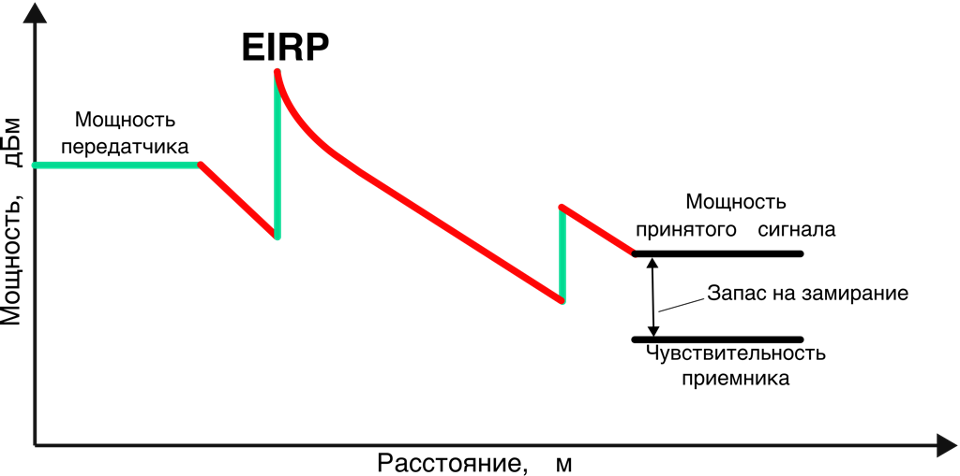
\includegraphics[width=1\textwidth]{link_power.png}
\caption{Энергетический потенциал линии связи.}
\label{fig:link_power}
\end{figure}

На стороне передатчика выходной мощностью является величина, равная мощности, подводимой к антенне. Данная величина из паспортной документации устройства имеет различные значения в зависимости от каждого поддерживаемого оборудованием стандарта и конкретных скоростей. В реальной условиях значения мощностей, как правило могут незначительно отклоняться от паспортных значений. Предельная мощность передатчика определяется государственными органами. Для примера, для БШС семейства протоколов IEEE 802.11 не превышает 100 мВт или, выражая в децибеллах, не боллее 20 дБм \cite{GKRCh18_13}.


Затухание сигнала могут происходить в кабелях антенны, зависящие от типа кабеля и рабочей частоты. При подключении антенны желательно обходиться минимальной длиной кабеля. Потери сигнала в антенном кабеле принимают $0, 1...2$ дБ/м. В технической документации в потерях кабеля также учтена величина затухания в кабельных разъемах. 

Усиление антенны описывает фокусирование переданного или полученного сигнала. Значения даны относительно полуволнового диполя или теоретического изотропного излучателя \cite{Gost62657}.

Мощность принимаемой антенны рассчитывается из уравнения передачи Фрииса:

\begin{displaymath}
  \label{eq:part3_Friis}
  \frac{P_{recv}}{P_{tr}} = G_{tr}G_{recv}\left(\frac{c}{4\pi R f} \right)^2,
\end{displaymath}
где
$c$ --  скорость света,
$f$ -- частота, 
$R$ рассточние между приемной и передающей антенной.


К потерям при распространении относятся все виды затухания сигнала, которые имеют место при его распространении от антенны передатчика к антенне приемника. Самая простая оценка потерь в свободном пространстве получается, если предположить, что сигналы передаются во всех направлениях, то есть мощность излучается одинаково во всех направлениях, и в зоне передачи или вокруг нее нет препятствий, которые могли бы повлиять на распространение электромагнитных сигналов \cite{Krouk2010}. Передающий сигнал рассеивается по мере увеличиня расстояния между приемником и передатчиком. Данный тип затухания называется потерями в свободном пространстве (Free Space Path Loss, $FSPL$).

Уравнение потерь в свободном пространстве ($FSPL$) при распространении между двумя антеннами в свободном пространстве (в воздухе):

\begin{equation}
  \label{eq:part3_FSPL}
  FSPL = \left(\frac{4\pi R f}{c} \right)^2.
\end{equation}

Формула \cref{eq:part3_FSPL}, выраженная в децибеллах будет выражаться как

\begin{equation}
  \label{eq:part3_L_fs}
  L_{fs} = 20 \lg{F} + 20\lg{R} + K,
  \end{equation}
где $F$ -- центральная частота, на котором работает канал связи, $R$ -- рассточние между приемной и передающей антенной и $K$ -- константа.

Константа $K$ зависит от размерностей частоты и расстояния:

\begin{itemize}
  \item для чистоты, выраженной в ГГц, и рассчтояния, выраженная в км, константа $K$ равна 92.45;
  \item для чистоты, выраженной в МГц, и рассчтояния, выраженная в км, константа $K$ равна 32.4;
  \item для чистоты, выраженной в МГц, и рассчтояния, выраженная в м, константа $K$ равна -27.55.
\end{itemize} 

Потери $L_{fs}$ выразим из уравнения энергетического потенциала канала связи \cref{eq:part3_link_budget} как:

\begin{equation}
  \label{eq:part3_L_fs_from_link_budget}
  L_{fs} = P_{tr} - L_{tr} + G_{tr} + G_{recv} - L_{recv} - SOM - P_{recv}.
\end{equation}


Запас на замирание сигнала, SOM,  учитывает все возможные факторы отрицательно влияющие на дальность связи. К таким факторам относятся:

\begin{itemize}
  \item температурный дрейф чувствительности приемника и выходной мощности передатчика;
  \item влияние погодных условий на передачу сигнала: туман, снег, дождь;
  \item  потери в антенно-фидерном тракте, возникающие из-за рассогласования фидера и антенны.
\end{itemize}
Приемник испытывает совокупное воздействие всех этих физических факторов, которые различаются в зависимости от положения приемника и передатчика в среде распространения. 

Минимальнная значения величины запаса на замирание  (System Operating Margin, $SOM$) должна быть не меньше  10 дБ. Считается, что 10-ти децибельный запас по усилению достаточен для инженерного расчета, но на практике зачастую используют значение $20 ... 30$ дБ \cite{Proletarsky}.

% \fixme{Энергетический потенциал указывает на качество канала передачи радиосигналов}.



% The Free Space Path Loss ($ FSPL $) equation defines the propagation signal loss between two antennas through free space (air):



Максимально возможную дальность связи между приемником и передатчиком выводится из уравнений \cref{eq:part3_L_fs} и \cref{eq:part3_L_fs_from_link_budget}:

\begin{equation}
  \label{eq:part3_D}
  R = 10^{\left(\frac{L_{fs} - 20\lg{F} - K}{20}\right)}.
\end{equation}

Используя формулу \cref{eq:part3_D} и \cref{eq:part3_L_fs_from_link_budget}, мы можем расчитать теоретическое максимальную дальность связи $ R_{jq}$ между базовыми станциями и радиусом покрытия $ r_j $ с предположением об отсутствии препятствий, отражений, влияния контуров местности и т. д. Это допущение приемлемо для нашего случая с открытой местностью.

\begin{figure}[h!]
  \centering
   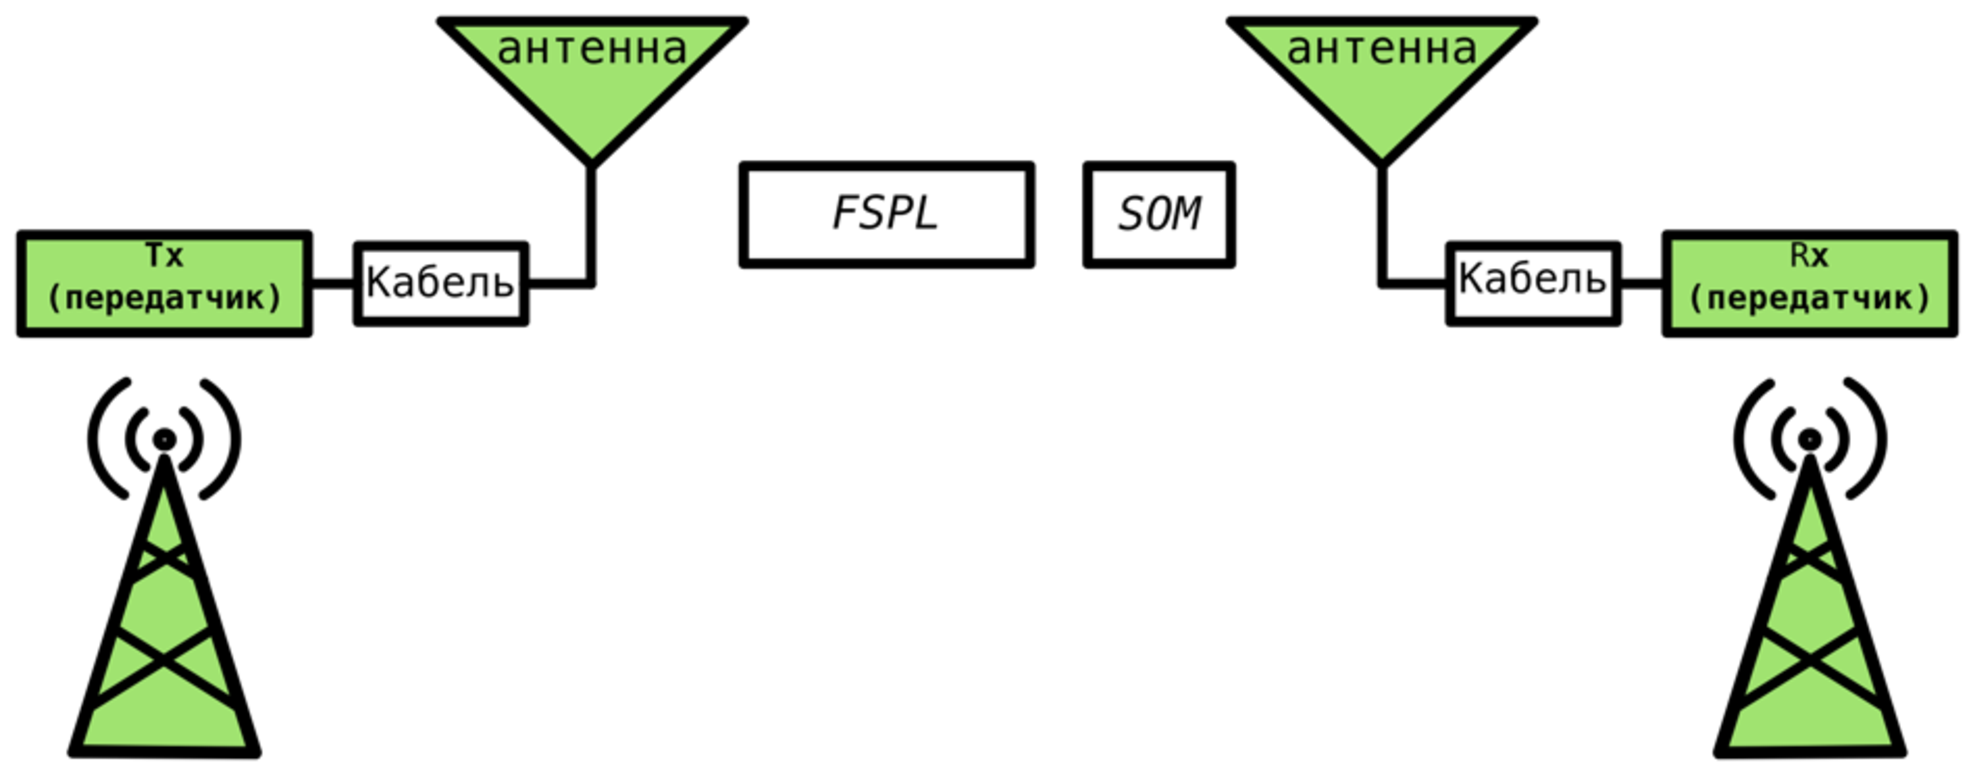
\includegraphics[width=0.8\textwidth]{link_distance.pdf}
\caption{Соединение между станциями.}
\label{fig:part3_link_distance}
\end{figure}

Для расчета дальности связи $R_{jq}$ (Рисунок \cref{fig:part3_link_distance}), базовые станции $s_j$ и $s_q$ будут рассматриваться как станции \textit{передатчик} и \textit{приемник}, соответственно. Будем считать, что станции оборудованы направленными антеннами с усилениями $G_{tr}^{R}$ и $G_{recv}^{R}$.

\begin{figure}[h!]
  \centering
   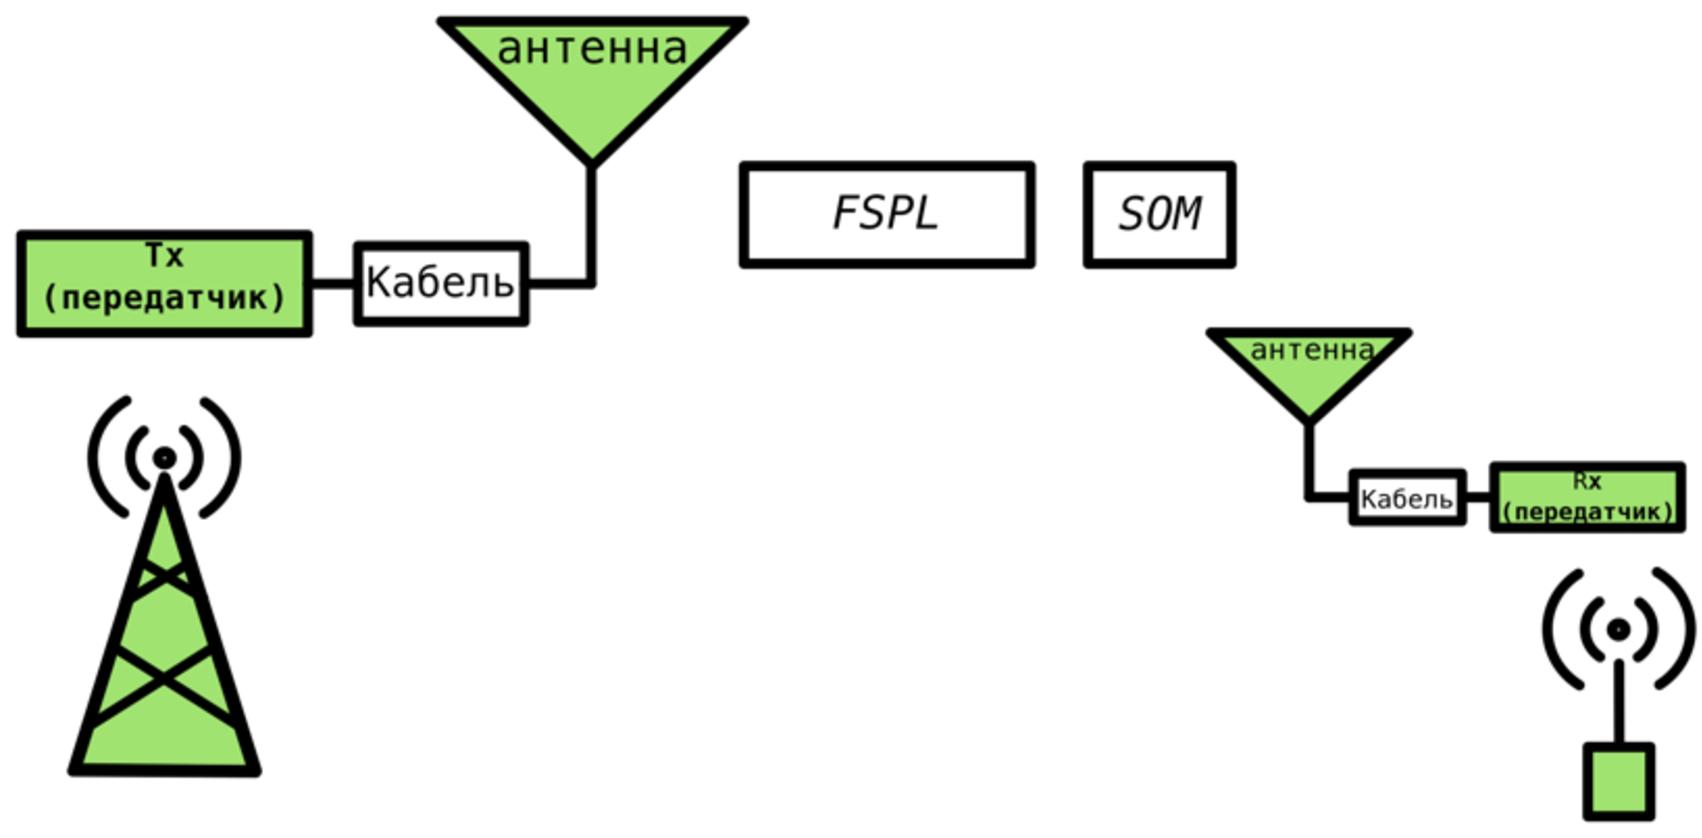
\includegraphics[width=0.8\textwidth]{coverage.pdf}
\caption{Покрытие станции}
\label{fig:part3_coverage}
\end{figure}

Каждая базовая станция оснащена всенаправленной антенной с заданным усилением антенны $G_ {tr}^{r}$. Данная антенн необходимо для покрытия заданной области.

% Each base station is equipped with an omnidirectional antenna with given gain antenna $G_{tr}^{r}$. A station uses this antenna to cover a given area.

При вычислении радиуса покрытия $r_j$ (Рисунок  \cref{fig:part3_coverage}) базовая станция будем считать \textit{передатчиком}, а пользовательское устройство \textit{приемником}.

\subsection{Расчет межконцевой задержки}\label{part4_e2e_delay_section}

Как уже было отмечено ранее, одним из важных ключевых задач при проектировании БШС является оценка ее характеристик производительности для удовлетворения требуемого качества обслуживания (quality of service, QoS). Одной из основных характеристик проектируемой сети является ее межконцевая задержка \cite{Vishnevsky2016_Methods_of_performance, Wang2017, Liu2016, Chen2019, Hosni2017, Capone2019, Abbas2017, Seliem2019, Malandra2018, Kalor2018, Larionov2019, Gao2016}. Для расчета сквозной задержки сети используют стохастические модели массового обслуживания \cite{Vishnevsky2016_Methods_of_performance, Wang2017, Liu2016, Malandra2018, Larionov2019, Gao2016}. 

Пусть задан частной случай БШС. Все БС связаны последовательно между собой в сеть с линейной топологией. Для расчета межконцевой задержки в простейшем случае рассмотрим беспроводную сеть как сеть массового обслуживания (СеМО) с кросс-трафиком и узлами $M/M/1$ (Рисунок \cref{fig:tandem_queue}). 

Узлами сети являются БС. Согласно символике Дж. Кендала, обозначение $M$ указывает на показательное распределение случайной величины \cite{VishnevskyBook, Kleinrock1975}. Каждая такая БC характеризуется случайными величинами входящего потоком пакетов и временем их обслуживания, принадлежащие экспоненциальному закону распределения. Каждый узел имеет один обслуживающий прибор. Для такой СеМО принято допущение о бесконечном размере буфера, в котором пакеты ожидают своего обслуживания. Данное допущение позволяет получить аналитическое решение, которое возможно использовать для проивзольного размера СеМО для данной топологии.

\begin{figure}[h!]
  \centering
   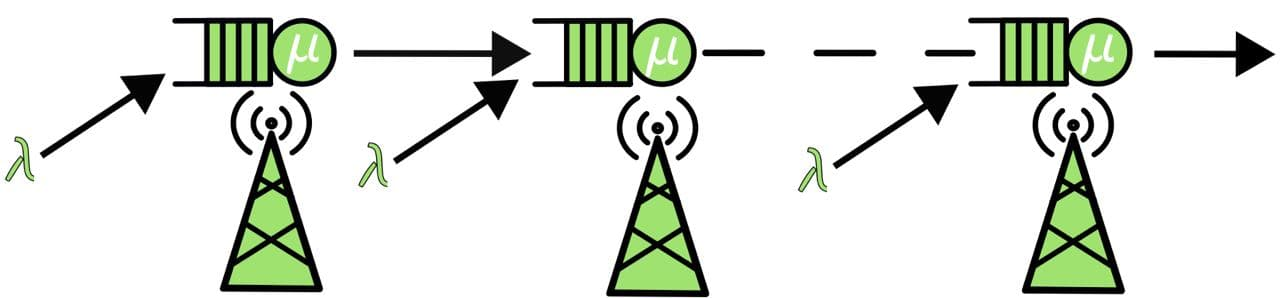
\includegraphics[width=1\textwidth]{tandem_queue.png}
\caption{СеМО с кросс-трафиком и узлами $M/M/1$.}
\label{fig:tandem_queue}
\end{figure}

На вход каждой станции поступает пуассоновский поток. Пуассоновский процесс представляет собой случайный процесс, характеризующийся  экспоненциально распределенным временем между событиями. Это один из наиболее важных случайных процессов в теории вероятностей, который широко используется для моделирования поведения трафика и входов во многих коммуникационных сетях и системах \cite{Kalor2018, Gao2016, Malandra2018, Seliem2019}. 

В пуассоновском процессе события происходят непрерывно и независимо друг от друга. Функция распределения имеет вид  \cite{VishnevskyBook, Kleinrock1975}:

\begin{displaymath}
P(X<x) = 
  \begin{cases}
    1 - e^{- \lambda x}, \quad x \geqslant 0; \\
    0, \quad x < 0.\\
  \end{cases}
\end{displaymath}

Для входящего потока интервалы между поступлениями заданны случайной величиной c экспоненциальным распределением и интенсивностью $\lambda$. Время обслуживания на узле задана также эскпоненциальным распределением и интенсивностью $\mu$. 


По теореме Бурке \cite{Burke1956}, поток на выходе узла $M/M/1$, а значит на входе каждой последующей фазы тоже пуассоновский. Интенсивность на выходе каждой фазы равна суммарной интенсивности всех входящих потоков с интенсивностями $\lambda$.

Пропускная способность на практике часто составляет половину от заданной в спецификации оборудования \cite{Proletarsky, Vladimirov2019}. Интенсивность времени обслуживания рассчитывается по формуле: 

\begin{displaymath}
    \mu_j = 0.5 \cdot p_j / w,
\end{displaymath}
где: $p_j$ - пропускная способность $j$-ой станции, Мбит/с; $w$ - средний размер пакета, Мбит.

Для каждой станции коэффициент загрузки равен:


\begin{displaymath}
\rho_j= \frac{\sum{\lambda}}{\mu_j} = \frac{q \cdot \lambda}{\mu_j} <1,
\end{displaymath}
где $q$ -- число входящих потоков. Условие $\rho_j<1$ является необходимым и достаточным условием существования стационарного режима функционирования СеМО.

Далее по формуле Литтла \cite{Little1961} можно рассчитать время задержки на каждой станции:

\begin{displaymath}
    \overline{T_j} = \frac{\rho_j}{1 - \rho_j} \cdot \frac{1}{q \cdot \lambda}.
\end{displaymath}

Тогда межконцевая задержки в сети равна

\begin{equation}
    \label{eq:end_to_end_delay}
    \overline{T}= \sum{\overline{T_j}}.
\end{equation}


Существуют более сложные модели очередей для оценок характеристик с более сложными распределения входящего трафика и времени обслуживания. Адекватные оценки дают модели с коррелированными входным потоком \cite{Vishnevsky2016_Methods_of_performance, Larionov2019}. К сожалению, такие модели труднорешаемы и для большего числа фаз СеМО не имеют аналитических расчетов. В данном исследовании будем использовать простейшую модель СеМО с узлами $M/M/1$ на этапе задачи оптимального размещения. Согласно предложенной концепции проектирования, полученную БШС с размещенными БС и выбранным техническим оборудованием можно будет в дальнейшем проводить на более сложных моделей на следующем этапе моделирования сети. Этот этап включает в себя математическое, имитационное моделирования для оценок характеристик производительности как время задержек, длины чередей, пропускная способность, вероятность потери пакетов и др. Данный этап позволяет провести комплексную проверку соотвествия QoS для полученного размещения БС.

\section{Выводы по главе \cref{ch:ch1}}

В главе представлено актуальность внедрения БШС в рамках цифровой трансформации нефтегазового сектора <<Индустрия 4.0>>. Представлены тематика исследования и задачи, затронутые в диссертации в рамках данного внедрения, а именно задачи синтеза топологии при проектировании беспроводных телекоммуникации на месторождении. Представлена структура последовательностей этапов при проектировании и место задачи синтеза в ней. Представлены методика расчета параметров БС необходимых в дальнейшем для оптимизационных задач размещения БС. 

% \begin{figure}[h!]
%   \centering
%    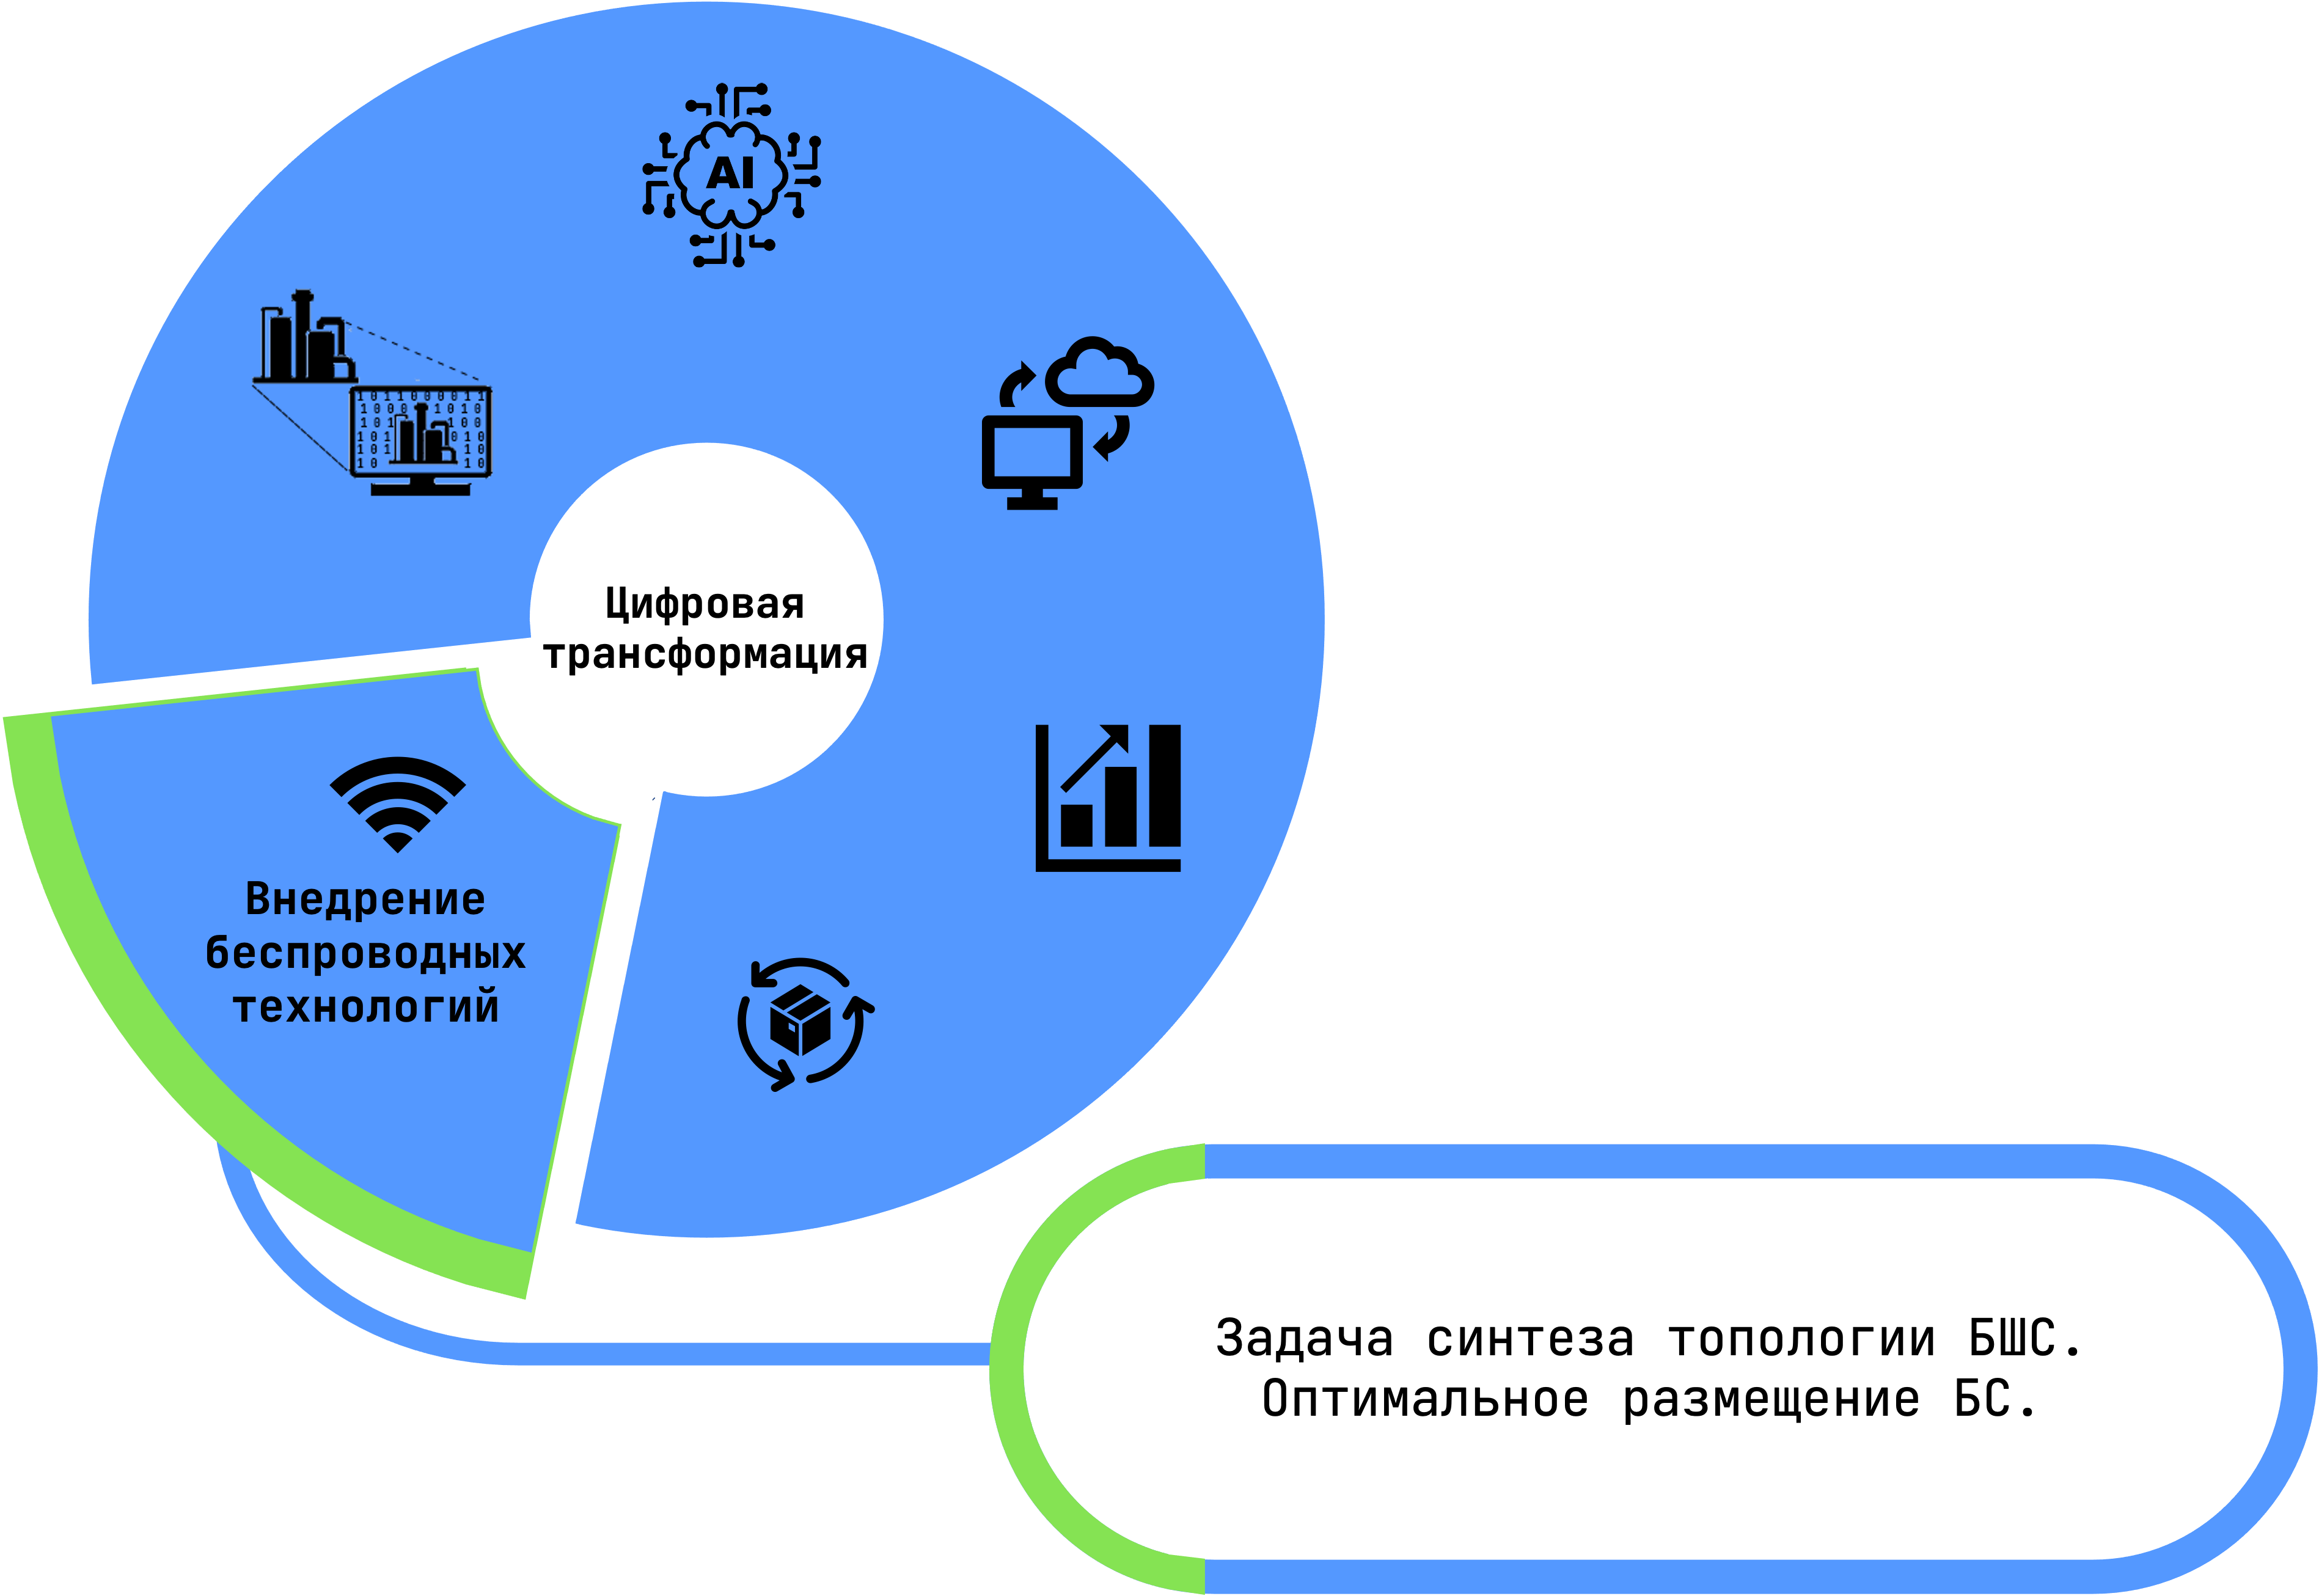
\includegraphics[width=1\textwidth]{industry4.png}
% \caption{Задача синтеза топологии при проектировании БШС в рамках цифровой трансформации "Индустрия 4.0".}
% \label{fig:industry4}
% \end{figure}





\FloatBarrier
